\chapter{Contador Ascendente}
El circuito electr\'onico de un contador est\'a compuesto por flip flops tipo T ya que estos pueden almacenar un bit el cual se lo llama estado y proporcionan la facilidad de invertir el estado cuando ocurre el evento del flanco ascendente del clock. Es decir, se produce un toggle.
\section{Funcionamiento Lógico del Contador Ascendente}
El funcionamiento lógico del contador se lo explica en la siguiente tabla:
\begin{center}
	\begin{table}[h!]
		\begin{center}
			\caption{Tabla de Verdad del Contador (3 bits)}
			\begin{tabular}{|c|c|}
				\hline
				%\textbf{INPUT} & \textbf{OUTPUT} \\
				%\hline
				\textbf{Clock Cycle} & \textbf{Q2 Q1 Q0} \\
				\hline
				0 & 0 0 0\\
				\hline
				1 & 0 0 1\\
				\hline
				2 & 0 1 0\\
				\hline
				3 & 0 1 1\\
				\hline
				4 & 1 0 0\\
				\hline
				5 & 1 0 1\\
				\hline
				6 & 1 1 0\\
				\hline
				7 & 1 1 1\\
				\hline
				8 & 0 0 0\\
				\hline
			\end{tabular} \\
		\end{center}
	\end{table}
\end{center}
Donde el clock cycle simboliza el número de flancos ascendentes que se van presentando. Y siendo Q2, Q1 y Q0 los estados que cada flip flop almacena.

\section{Tipos de Contadores}
Los dos tipos básicos de contadores son el sincrónico y al asincrónico. A continuación se muestran los circutios electrónicos de cada uno.

\begin{center}
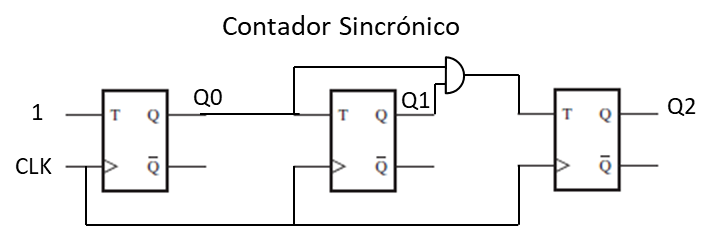
\includegraphics{../7-Async-Sync-Counter/contador sinc.png}
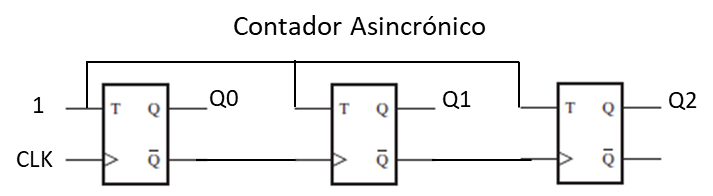
\includegraphics{../7-Async-Sync-Counter/contador asinc.png}
\end{center}

\subsection{Análisis de Ambos Circuitos}

Para poder analizar ambos circuitos, se implementó el circuito en una placa impresa (PCB) y se hizo uso de leds para hacer el circutio más interactivo.
A continuación se muestra el circuito en físico:

\begin{center}
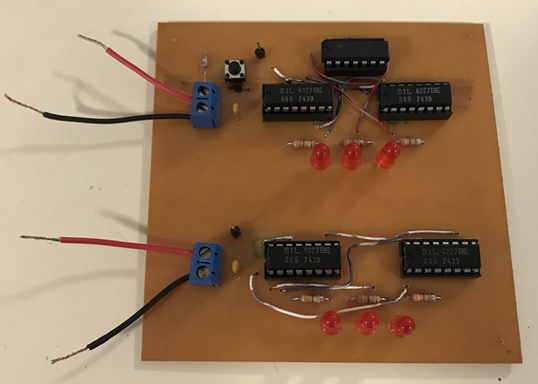
\includegraphics{../7-Async-Sync-Counter/pcb.png}
\end{center}

Luego se procedió a medir utilizando el osciloscopio la entrada (clock) y las salidas de cada estado. Y se obtuvo lo siguiente para ambos contadores:

\begin{center}
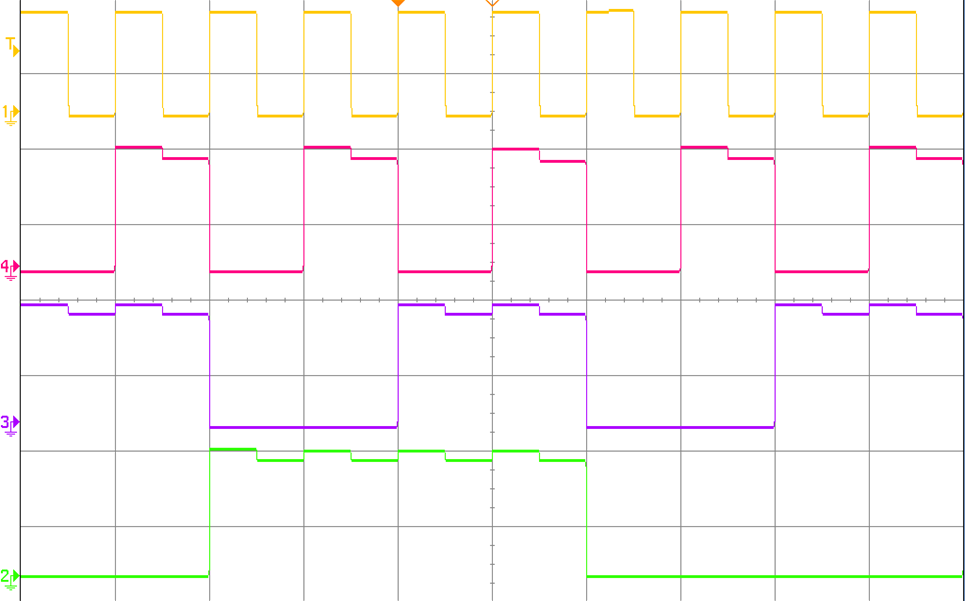
\includegraphics{../7-Async-Sync-Counter/contador osc.png}
\end{center}

Siendo la señal amarilla el clock, la señal roja el estado Q0, la señal violeta el estado Q1 y la señal verde el estado Q2.
Al hacer zoom modificando la escala del tiempo en la zona donde se encuentra el flanco ascendente del clock, se puede ver lo siguiente:

\begin{center}
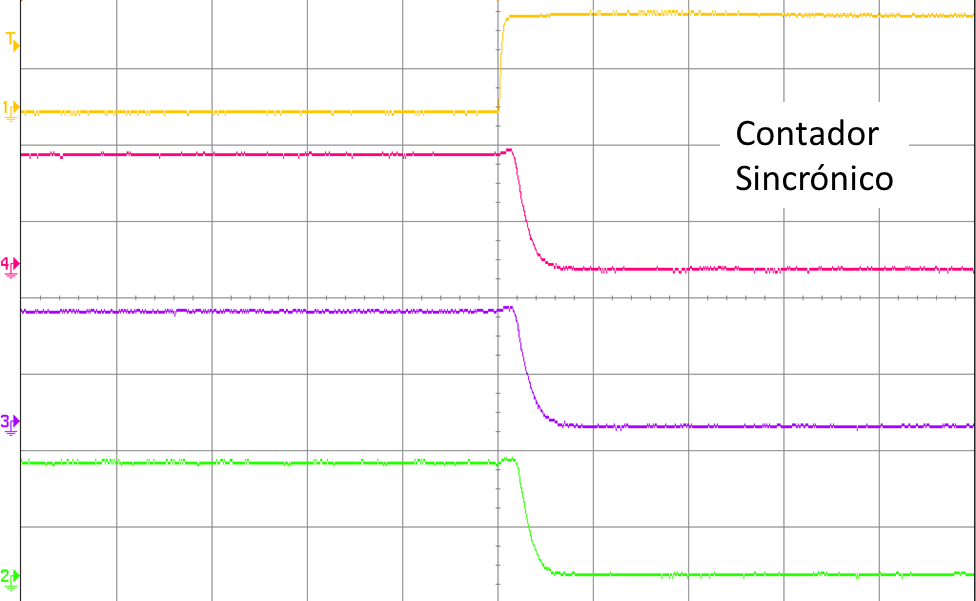
\includegraphics{../7-Async-Sync-Counter/counter_s2.png}
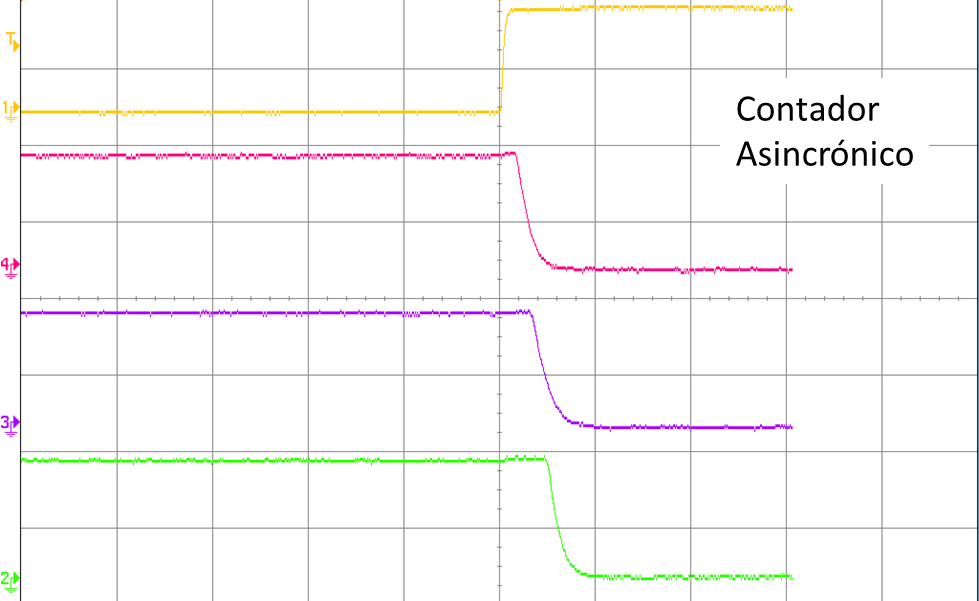
\includegraphics{../7-Async-Sync-Counter/counter_a2.png}
\end{center}

Se puede observar que en el contador sicrónico, los estados presentan un tiempo de propagación similar debido a que los flip flops tienen el mismo clock como input, es decir, están sincronizados.
En cambio en el contador asincrónico, como los flip flops no están sincronizados, los timpos de propagación se van sumando. Razón por la cual el estado Q2 es el último en establecerse.

\subsection{Conclusión}
En conclusión se puede decir que el contandor sincrónico es más rápido que en asincrónico. Además en contador asincrónico puede presentar problemas si el tiempo de propagación total es mayor que el tiempo entre flancos ascendentes del clock.